\documentclass{beamer}
\usepackage[utf8]{inputenc}
\usepackage[french]{babel}
\usepackage{lmodern}
\usepackage{amsmath}
\usepackage{amssymb}
\usepackage{pgf,tikz}
\usepackage{graphicx}
\usepackage{stmaryrd}
\usepackage[export]{adjustbox}

\usetheme{Warsaw}
\title[Analyse de sentiment]{Analyse de sentiment}
\author{Frédéric Wantiez et Pierre Vigier}
\institute{Supélec - Projet de synthèse}
\date{15 juin 2016}
\begin{document}

\begin{frame}
\titlepage
\end{frame}

\AtBeginSubsection[]
{
 \begin{frame}<beamer>
   \frametitle{Plan}
   \tableofcontents[currentsection,currentsubsection]
 \end{frame}
}

\begin{frame}{Introduction}
\begin{block}{Définition}
L'analyse de sentiments consiste à dire si un texte dégage un sentiment positif ou négatif.
\end{block}

\begin{block}{Applications}
Les principales applications de l'analyse de sentiments sont :
\begin{itemize}
	\item en marketing : repérer les promoteurs et les détracteurs ;
	\item en finance : miner les réseaux sociaux et les blogs pour prédire les mouvements de marché et la popularité d'un produit.
\end{itemize}
\end{block}
\end{frame}

\tableofcontents

\section{Description du problème}

\subsection{Présentation du problème}

\begin{frame}
\begin{block}{Notations}
Nous noterons :
\begin{itemize}
	\item $V=\{w_{1}, ..., w_{D}\}$ : l'ensemble de tous les mots ;
	\item $V^{*}=\cup_{n \geq 0}{V^{n}}$ : l'ensemble de tous les textes sur le vocabulaire $V$;
	\item $x_{1}, ..., x_{N} \in V^{*}$ : les textes de notre ensemble de de données ;
	\item $y_{1}, ..., y_{N} \in \{0, 1\}$ : les sentiments associés à chaque texte.
\end{itemize}
\end{block}
\end{frame}

\begin{frame}
\begin{block}{Formalisation}
Notre objectif est de déterminer une fonction $f$ telle que : 
$$
\forall i \in {1, ..., N}, y_{i} \approx \hat{y}_{i} = f(x_{i})
$$
\end{block}

\begin{block}{Mesure de performance}
Nous allons utiliser la précision comme mesure de performance, nous la définissions telle que :
$$
A(y_{1}, ..., y_{N}, \hat{y}_{1}, ..., \hat{y}_{N}) = \frac{\sum_{i=0}^{N}{1_{y_{i}=\hat{y}_{i}}}}{N}$$
\end{block}
\end{frame}

\subsection{Ensemble de données}

\begin{frame}
\begin{block}{Exemple d'avis négatif}
\texttt{Story of a man who has unnatural feelings for a pig. Starts out with a opening scene that is a terrific example of absurd comedy. A formal orchestra audience is turned into an insane, violent mob by the crazy chantings of it's singers. Unfortunately it stays absurd the WHOLE time with no general narrative eventually making it just too off putting. Even those from the era should be turned off. The cryptic dialogue would make Shakespeare seem easy to a third grader. On a technical level it's better than you might think with some good cinematography by future great Vilmos Zsigmond. Future stars Sally Kirkland and Frederic Forrest can be seen briefly.}
\end{block}
\end{frame}

\begin{frame}
\begin{block}{Exemple d'avis positif}
\texttt{The plot had some wretched, unbelievable twists. However, the chemistry between Mel Brooks and Leslie Ann Warren was excellent. The insight that she comes to, ""There are just moments,"" provides a philosophical handle by which anyone could pick up, and embrace, life.<br /><br />That was one of several moments that were wonderfully memorable.}
\end{block}
\end{frame}

\section{Premiers essais}

\subsection{Sacs de mots}

\begin{frame}{Définitions}
\begin{block}{Nombre d’occurrences d'un mot}
Pour un texte $t \in V^{*}$, posons :
$$
\forall i \in \{1, ..., D\}, tf_{i,t} = card(\{j, t_{j}=w_{i}\})
$$
\end{block}

\begin{block}{Sac de mots}
Le sac de mot d'un texte $t$ est un vecteur $b$ de $\mathbb{R}^{D}$ tel que :
$$
\forall i \in {1, ..., D}, b_{i} = tf_{i,t}
$$
\end{block}
\end{frame}

\begin{frame}{Exemple}
\begin{align*}
S_{1} & = "\text{Bob aime les films d'action.}" \\
S_{2} & = "\text{Alice préfère les films d'amour.}"
\end{align*}
Le vocabulaire commun aux deux phrases est :
$$
V = \{\text{Bob}, \text{aime}, \text{les}, \text{films}, \text{d}, \text{action}, \text{Alice}, \text{préfère}, \text{amour}\}
$$
Sacs de mots associés à $S_{1}$ et $S_{2}$ :
\begin{align*}
b_{1} & = (1, 1, 1, 1, 1, 1, 0, 0, 0)^{T} \\
b_{2} & = (0, 0, 1, 1, 1, 0, 1, 1, 1)^{T}
\end{align*}
\end{frame}

\begin{frame}{TF-IDF}
\begin{block}{Fréquence inverse de document}
La fréquence inverse de document du mot $w_{i}$ est définie par :
$$
idf_{i} = log(\frac{N}{N_{i}})
$$
\end{block}

\begin{block}{Sac de mots pondéré}
Le sac de mot pondéré d'un texte $t$ est un vecteur $b$ de $\mathbb{R}^{D}$ tel que :
$$
\forall i \in {1, ..., D}, b_{i} = tf_{i,t} \times idf_{i}
$$
\end{block}
\end{frame}

\begin{frame}{Résultats}
\begin{figure}
\begin{center}
\begin{tabular}{|l|c|}
	\hline
	Forêt aléatoire à 100 estimateurs + BOW & 0.84356 \\
	\hline
	Forêt aléatoire à 100 estimateurs + BOW + TF-IDF & 0.83952 \\
	\hline
	Régression logistique + BOW & 0.84748 \\
	\hline
	Régression logistique + BOW + TF-IDF & 0.88308 \\
	\hline
\end{tabular}
\caption{Précisions des sacs de mots avec différents algorithmes (BOW : sacs de mots, TF-IDF : sacs de mots pondérés par IDF)}
\end{center}
\end{figure}
\end{frame}

\begin{frame}{Régression logistique}
\begin{figure}
\begin{center}
% Graphic for TeX using PGF
% Title: /home/pierre/Programming/sa/report/images/lr_net.dia
% Creator: Dia v0.97.3
% CreationDate: Mon May 30 20:31:12 2016
% For: pierre
% \usepackage{tikz}
% The following commands are not supported in PSTricks at present
% We define them conditionally, so when they are implemented,
% this pgf file will use them.
\ifx\du\undefined
  \newlength{\du}
\fi
\setlength{\du}{15\unitlength}
\begin{tikzpicture}[scale=0.6]
\pgftransformxscale{1.000000}
\pgftransformyscale{-1.000000}
\definecolor{dialinecolor}{rgb}{0.000000, 0.000000, 0.000000}
\pgfsetstrokecolor{dialinecolor}
\definecolor{dialinecolor}{rgb}{1.000000, 1.000000, 1.000000}
\pgfsetfillcolor{dialinecolor}
\definecolor{dialinecolor}{rgb}{1.000000, 1.000000, 1.000000}
\pgfsetfillcolor{dialinecolor}
\pgfpathellipse{\pgfpoint{18.500000\du}{9.500000\du}}{\pgfpoint{1.500000\du}{0\du}}{\pgfpoint{0\du}{1.500000\du}}
\pgfusepath{fill}
\pgfsetlinewidth{0.100000\du}
\pgfsetdash{}{0pt}
\pgfsetdash{}{0pt}
\definecolor{dialinecolor}{rgb}{0.000000, 0.000000, 0.000000}
\pgfsetstrokecolor{dialinecolor}
\pgfpathellipse{\pgfpoint{18.500000\du}{9.500000\du}}{\pgfpoint{1.500000\du}{0\du}}{\pgfpoint{0\du}{1.500000\du}}
\pgfusepath{stroke}
\definecolor{dialinecolor}{rgb}{1.000000, 1.000000, 1.000000}
\pgfsetfillcolor{dialinecolor}
\pgfpathellipse{\pgfpoint{18.500000\du}{13.500000\du}}{\pgfpoint{1.500000\du}{0\du}}{\pgfpoint{0\du}{1.500000\du}}
\pgfusepath{fill}
\pgfsetlinewidth{0.100000\du}
\pgfsetdash{}{0pt}
\pgfsetdash{}{0pt}
\definecolor{dialinecolor}{rgb}{0.000000, 0.000000, 0.000000}
\pgfsetstrokecolor{dialinecolor}
\pgfpathellipse{\pgfpoint{18.500000\du}{13.500000\du}}{\pgfpoint{1.500000\du}{0\du}}{\pgfpoint{0\du}{1.500000\du}}
\pgfusepath{stroke}
\definecolor{dialinecolor}{rgb}{1.000000, 1.000000, 1.000000}
\pgfsetfillcolor{dialinecolor}
\pgfpathellipse{\pgfpoint{18.500000\du}{20.500000\du}}{\pgfpoint{1.500000\du}{0\du}}{\pgfpoint{0\du}{1.500000\du}}
\pgfusepath{fill}
\pgfsetlinewidth{0.100000\du}
\pgfsetdash{}{0pt}
\pgfsetdash{}{0pt}
\definecolor{dialinecolor}{rgb}{0.000000, 0.000000, 0.000000}
\pgfsetstrokecolor{dialinecolor}
\pgfpathellipse{\pgfpoint{18.500000\du}{20.500000\du}}{\pgfpoint{1.500000\du}{0\du}}{\pgfpoint{0\du}{1.500000\du}}
\pgfusepath{stroke}
% setfont left to latex
\definecolor{dialinecolor}{rgb}{0.000000, 0.000000, 0.000000}
\pgfsetstrokecolor{dialinecolor}
\node at (18.500000\du,17.100000\du){...};
\definecolor{dialinecolor}{rgb}{1.000000, 1.000000, 1.000000}
\pgfsetfillcolor{dialinecolor}
\pgfpathellipse{\pgfpoint{32.500000\du}{15.000000\du}}{\pgfpoint{1.500000\du}{0\du}}{\pgfpoint{0\du}{1.500000\du}}
\pgfusepath{fill}
\pgfsetlinewidth{0.100000\du}
\pgfsetdash{}{0pt}
\pgfsetdash{}{0pt}
\definecolor{dialinecolor}{rgb}{0.000000, 0.000000, 0.000000}
\pgfsetstrokecolor{dialinecolor}
\pgfpathellipse{\pgfpoint{32.500000\du}{15.000000\du}}{\pgfpoint{1.500000\du}{0\du}}{\pgfpoint{0\du}{1.500000\du}}
\pgfusepath{stroke}
\pgfsetlinewidth{0.100000\du}
\pgfsetdash{}{0pt}
\pgfsetdash{}{0pt}
\pgfsetbuttcap
{
\definecolor{dialinecolor}{rgb}{0.000000, 0.000000, 0.000000}
\pgfsetfillcolor{dialinecolor}
% was here!!!
\pgfsetarrowsend{stealth}
\definecolor{dialinecolor}{rgb}{0.000000, 0.000000, 0.000000}
\pgfsetstrokecolor{dialinecolor}
\draw (20.000000\du,9.500000\du)--(31.000000\du,15.000000\du);
}
\pgfsetlinewidth{0.100000\du}
\pgfsetdash{}{0pt}
\pgfsetdash{}{0pt}
\pgfsetbuttcap
{
\definecolor{dialinecolor}{rgb}{0.000000, 0.000000, 0.000000}
\pgfsetfillcolor{dialinecolor}
% was here!!!
\pgfsetarrowsend{stealth}
\definecolor{dialinecolor}{rgb}{0.000000, 0.000000, 0.000000}
\pgfsetstrokecolor{dialinecolor}
\draw (20.000000\du,13.500000\du)--(31.000000\du,15.000000\du);
}
\pgfsetlinewidth{0.100000\du}
\pgfsetdash{}{0pt}
\pgfsetdash{}{0pt}
\pgfsetbuttcap
{
\definecolor{dialinecolor}{rgb}{0.000000, 0.000000, 0.000000}
\pgfsetfillcolor{dialinecolor}
% was here!!!
\pgfsetarrowsend{stealth}
\definecolor{dialinecolor}{rgb}{0.000000, 0.000000, 0.000000}
\pgfsetstrokecolor{dialinecolor}
\draw (20.000000\du,20.500000\du)--(31.000000\du,15.000000\du);
}
% setfont left to latex
\definecolor{dialinecolor}{rgb}{0.000000, 0.000000, 0.000000}
\pgfsetstrokecolor{dialinecolor}
\node at (18.500000\du,9.722500\du){$b_{1}$};
% setfont left to latex
\definecolor{dialinecolor}{rgb}{0.000000, 0.000000, 0.000000}
\pgfsetstrokecolor{dialinecolor}
\node at (18.500000\du,13.722500\du){$b_{2}$};
% setfont left to latex
\definecolor{dialinecolor}{rgb}{0.000000, 0.000000, 0.000000}
\pgfsetstrokecolor{dialinecolor}
\node[anchor=west] at (17.000000\du,21.000000\du){};
% setfont left to latex
\definecolor{dialinecolor}{rgb}{0.000000, 0.000000, 0.000000}
\pgfsetstrokecolor{dialinecolor}
\node at (18.500000\du,20.722500\du){$b_{D}$};
% setfont left to latex
\definecolor{dialinecolor}{rgb}{0.000000, 0.000000, 0.000000}
\pgfsetstrokecolor{dialinecolor}
\node at (32.500000\du,15.222500\du){$\sigma$};
\pgfsetlinewidth{0.100000\du}
\pgfsetdash{}{0pt}
\pgfsetdash{}{0pt}
\pgfsetbuttcap
{
\definecolor{dialinecolor}{rgb}{0.000000, 0.000000, 0.000000}
\pgfsetfillcolor{dialinecolor}
% was here!!!
\pgfsetarrowsend{stealth}
\definecolor{dialinecolor}{rgb}{0.000000, 0.000000, 0.000000}
\pgfsetstrokecolor{dialinecolor}
\draw (20.000000\du,17.000000\du)--(31.000000\du,15.000000\du);
}
% setfont left to latex
\definecolor{dialinecolor}{rgb}{0.000000, 0.000000, 0.000000}
\pgfsetstrokecolor{dialinecolor}
\node[anchor=west] at (24.000000\du,11.200000\du){$\theta_{1}$};
% setfont left to latex
\definecolor{dialinecolor}{rgb}{0.000000, 0.000000, 0.000000}
\pgfsetstrokecolor{dialinecolor}
\node[anchor=west] at (26.000000\du,14.000000\du){};
% setfont left to latex
\definecolor{dialinecolor}{rgb}{0.000000, 0.000000, 0.000000}
\pgfsetstrokecolor{dialinecolor}
\node[anchor=west] at (24.000000\du,13.500000\du){$\theta_{2}$};
% setfont left to latex
\definecolor{dialinecolor}{rgb}{0.000000, 0.000000, 0.000000}
\pgfsetstrokecolor{dialinecolor}
\node[anchor=west] at (24.000000\du,15.500000\du){...};
% setfont left to latex
\definecolor{dialinecolor}{rgb}{0.000000, 0.000000, 0.000000}
\pgfsetstrokecolor{dialinecolor}
\node[anchor=west] at (24.000000\du,17.100000\du){$\theta_{D}$};
\end{tikzpicture}

\end{center}
\caption{Représentation d'une régression logistique sous forme de réseau.}
\end{figure}
\end{frame}

\begin{frame}[containsverbatim]{Mots négatifs}
\begin{verbatim}
NEGATIVE
1. worst (-9.207327806842622)
2. bad (-7.259958398881469)
3. awful (-6.415897979257145)
4. waste (-6.330645081158189)
5. boring (-5.972322478351235)
6. poor (-5.290181559864669)
7. terrible (-4.680185463018839)
8. worse (-4.432747319290786)
9. nothing (-4.411951085231576)
10. dull (-4.377273111550886)
\end{verbatim}
\end{frame}

\begin{frame}[containsverbatim]{Mots positifs}
\begin{verbatim}
POSITIVE
1. great (6.731768881148247)
2. excellent (6.010829696751981)
3. perfect (4.944364766157447)
4. best (4.721911978651118)
5. wonderful (4.516264655915644)
6. amazing (4.08891536519038)
7. today (3.6921102148583946)
8. favorite (3.658223120278884)
9. loved (3.589046275536792)
10. well (3.5422155660495744)
\end{verbatim}
\end{frame}

\subsection{Vecteurs de mots}

\begin{frame}{Modèle Skip-gram}
\begin{figure}
\begin{center}
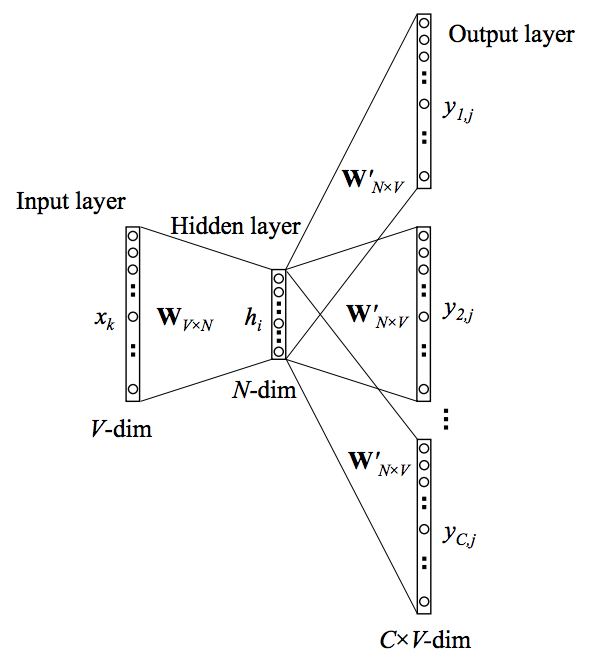
\includegraphics[scale=0.5]{images/skip_gram.png}
\caption{Réseau de neurones du modèle Skip-gram (source : Wikimedia).}
\label{skip_gram}
\end{center}
\end{figure}
\end{frame}

\begin{frame}{Visualisation t-SNE}
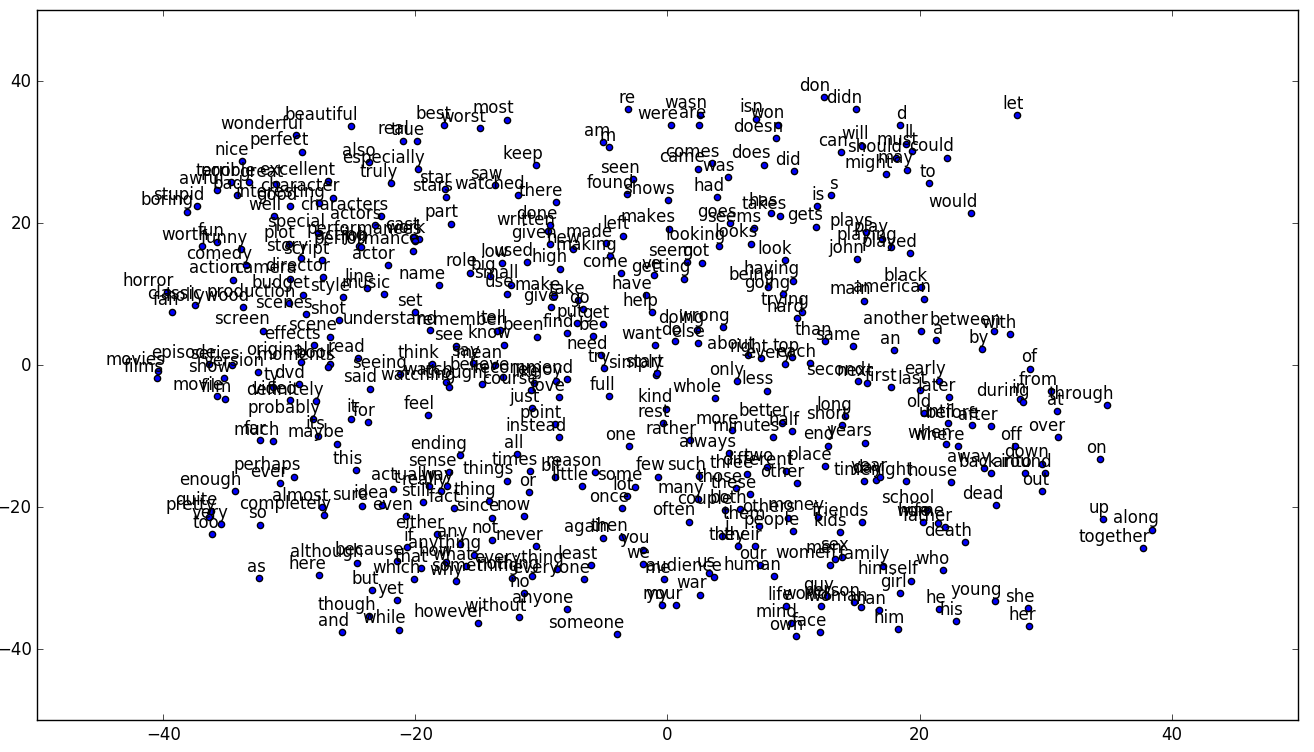
\includegraphics[scale=0.35]{images/tsne_plot.png}
\end{frame}

\begin{frame}{Cluster de mots liés au cinéma}
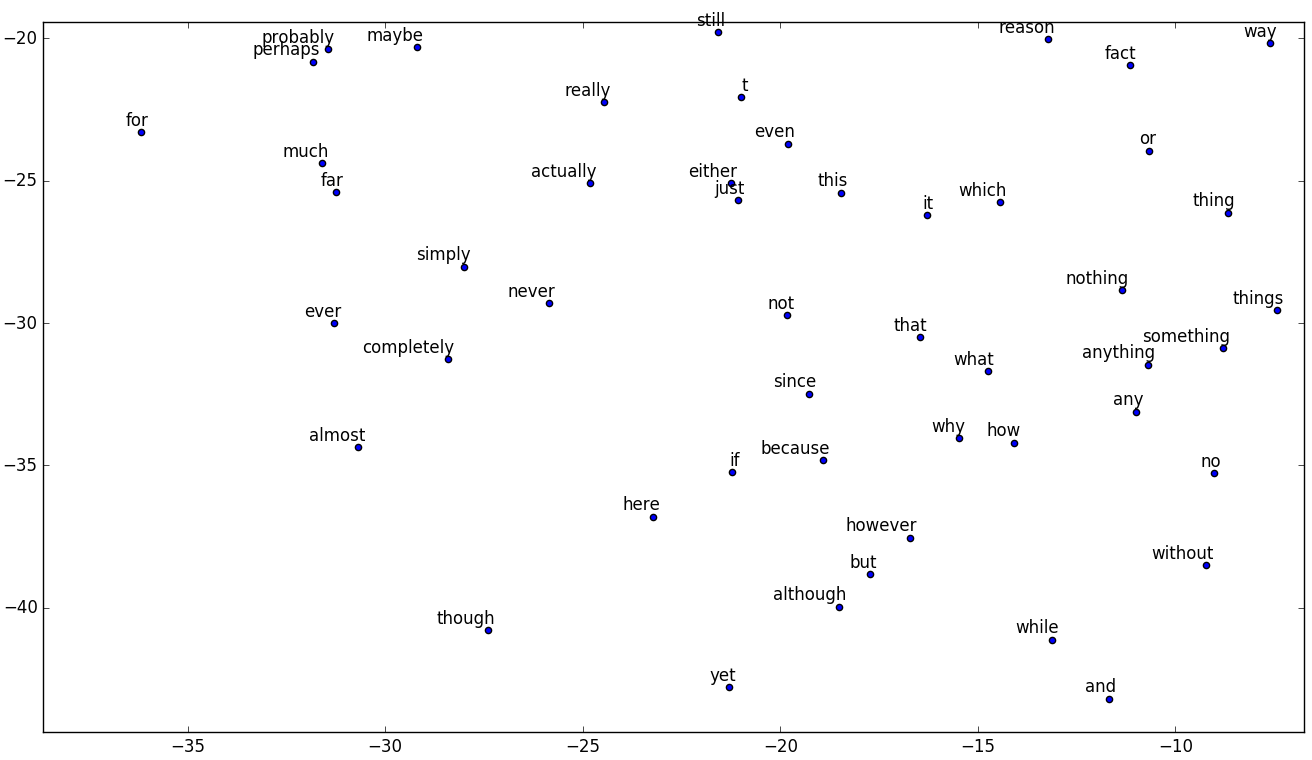
\includegraphics[scale=0.35]{images/cluster_cinema.png}
\end{frame}

\begin{frame}{Cluster de mots-outils}
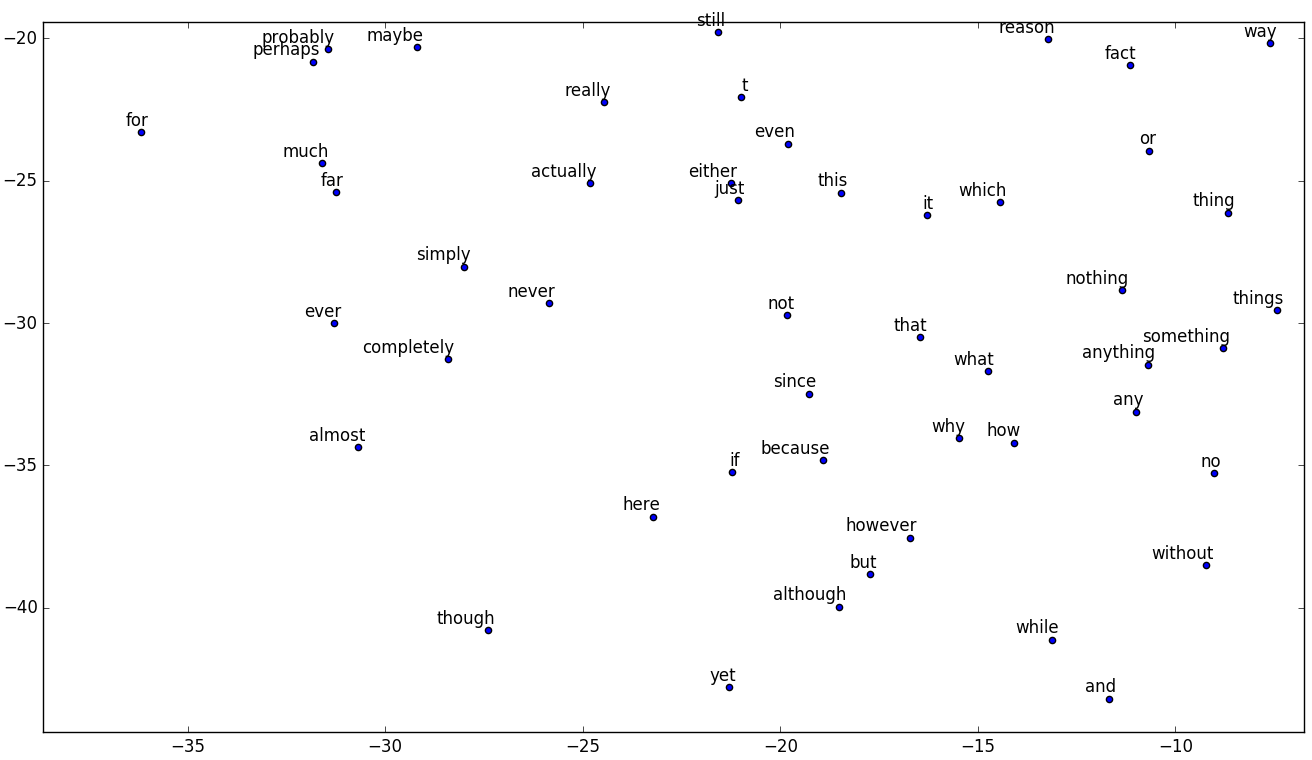
\includegraphics[scale=0.35]{images/cluster_toolwords.png}
\end{frame}

\begin{frame}{Vecteur d'un texte}
\begin{block}{Moyenne de vecteurs de mots}
Le vecteur représentant un texte $t$ est le vecteur :
$$
h_{vec}(t) = \frac{\sum_{w_{i} \in t}{tf_{i, t}v_{i}}}{\sum_{w_{i} \in t}{tf_{i, t}}} 
$$
\end{block}

\begin{block}{Moyenne pondérées de vecteurs de mots}
Le vecteur représentant un texte $t$ est le vecteur :
$$
h_{vec+idf}(t) = \frac{\sum_{w_{i} \in t}{tf_{i, t}idf_{i}v_{i}}}{\sum_{w_{i} \in t}{tf_{i, t}idf_{i}}}
$$
\end{block}
\end{frame}

\begin{frame}{Résultats}
\begin{figure}
\begin{center}
\begin{tabular}{|l|c|}
	\hline
	Forêt aléatoire à 100 estimateurs + Vec & 0.7954 \\
	\hline
	Forêt aléatoire à 100 estimateurs + Vec + TF-IDF & 0.79416 \\
	\hline
	Régression logistique + Vec & 0.81652 \\
	\hline
	Régression logistique + Vec + TF-IDF & 0.81688 \\
	\hline
\end{tabular}
\caption{Précisions des vecteurs de mot avec différents algorithmes (Vec : vecteurs de mots, TF-IDF : vecteurs de mot pondérés par IDF)}
\end{center}
\end{figure}
\end{frame}

\begin{frame}{Courbes d'apprentissage}
Courbe d'apprentissage pour les sacs de mots (à gauche) et les vecteurs de mot (à droite) :
\begin{center}
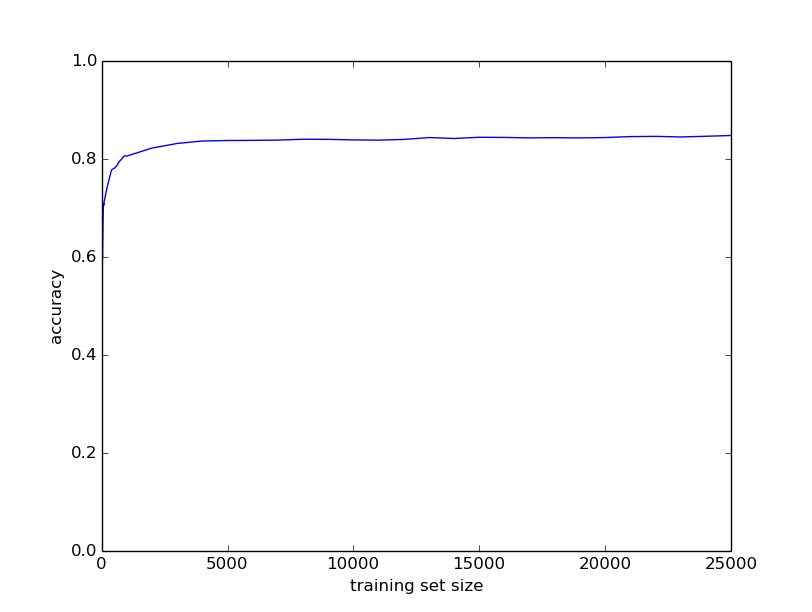
\includegraphics[scale=0.25]{images/learning_curve_lr_bow.png}
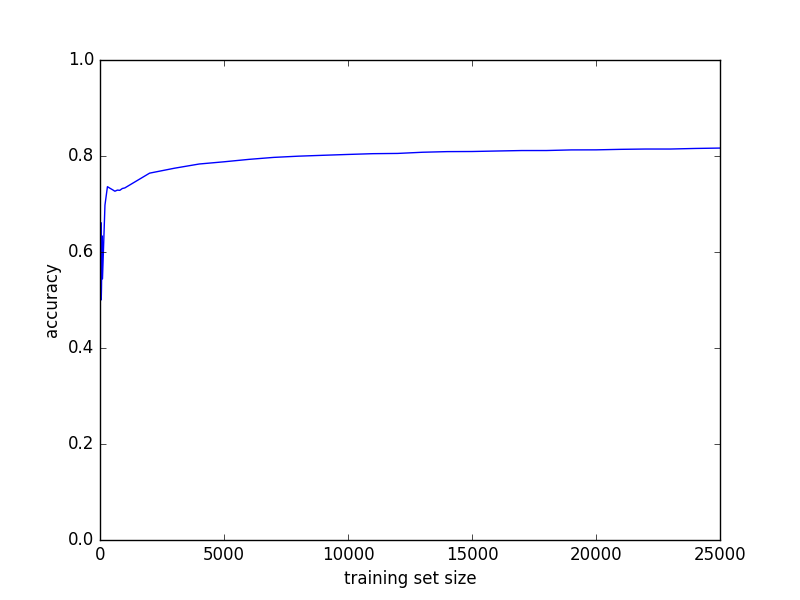
\includegraphics[scale=0.25]{images/learning_curve_lr_vec.png}
\end{center}
\end{frame}

\section{Prise en compte de l'ordre des mots}

\subsection{N-grammes}

\begin{frame}
\begin{block}{N-gramme}
Les n-grammes, $n \in \mathbb{N}$, d'un texte $t$ sont les n-uplets de mots consécutifs de $t$.
\end{block}

\begin{block}{Exemple}
Considérons la phrase $t="\text{Bob aime les films d'action.}"$, les bigrammes ou 2-grammes de $t$ sont :
$$
\{(\text{Bob}, \text{aime}), (\text{aime}, \text{les}), (\text{les}, \text{films}), (\text{films}, \text{d}), (\text{d}, \text{action})\}
$$
\end{block}
\end{frame}

\begin{frame}[containsverbatim]{Bigrammes les plus courants}
\begin{verbatim}
big_list.most_common(10)
[('ever seen', 1319),
 ('special effects', 1114),
 ('even though', 1043),
 ('one best', 919),
 ('low budget', 880),
 ('year old', 878),
 ('looks like', 838),
 ('waste time', 789),
 ('see movie', 772),
 ('much better', 746)]
\end{verbatim}
\end{frame}

\begin{frame}
\begin{figure}
\begin{center}
\begin{tabular}{|c|c|c|c|}
	\hline
	C & n & TF-IDF & Précision \\
	\hline
	5000 & 1 & Non & 0.85164 \\
	\hline
	10000 & 1 & Non & 0.85432 \\
	\hline
	15000 & 1 & Non & 0.85664 \\
	\hline
	\hline
	5000 & 2 & Non & 0.8582 \\
	\hline
	10000 & 2 & Non & 0.86844 \\
	\hline
	15000 & 2 & Non & 0.87544 \\
	\hline
	\hline
	5000 & 1 & Oui & 0.88308 \\
	\hline
	10000 & 1 & Oui & 0.88364 \\
	\hline
	15000 & 1 & Oui & 0.88412 \\
	\hline
	\hline
	5000 & 2 & Oui & 0.88848 \\
	\hline
	10000 & 2 & Oui & 0.89312 \\
	\hline
	15000 & 2 & Oui & 0.89432 \\
	\hline
	20000 & 2 & Oui & 0.8954 \\
	\hline
\end{tabular}
\caption{Précisions des sacs de n-grammes en entrée d'une régression logistique.}
\end{center}
\end{figure}
\end{frame}

\subsection{Vecteurs de paragraphe}
	
	\begin{frame}
	\begin{figure}
	\begin{center}
	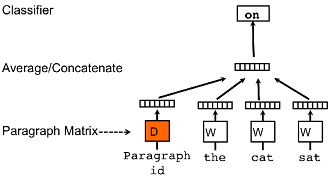
\includegraphics{images/paragraph_vectors.png}
	\caption{Framework d'apprentissage des paragraph vectors (source : Mikolov et al).}
	\label{paragraph_vectors}
	\end{center}
	\end{figure}
	\end{frame}
	
	\begin{frame}[containsverbatim]{Analyse sémantique du modèle}
	\begin{verbatim}
	In[1]: model.most_similar('interesting')
Out[1]:
('enjoyable', 0.549770712852478),
 ('entertaining', 0.5360784530639648),
 ('important', 0.5295416712760925),
 ('intriguing', 0.4986931085586548),
 ('amazing', 0.49587947130203247),
 ('exciting', 0.4942770004272461),
 ('excellent', 0.4942253828048706),
 ('awesome', 0.46036389470100403),
 ('amusing', 0.4536857306957245),
 ('impressive', 0.448122501373291)
	\end{verbatim}
	\end{frame}
	
	\begin{frame}
	\begin{table}
	\begin{tabular}{|l|c|}
	\hline
	Régression linéaire + PV-DM (concat.) & 0.883 \\
	\hline
	Régression linéaire + PV-DM (mean)  & 0.823 \\
	\hline
\end{tabular}
\caption{Précision des paragraph vectors avec les deux variantes utilisées pour des vecteurs de dimension 300}
\label{results_pv}
	\end{table}
	\end{frame}
	
	\begin{frame}
	\begin{figure}[h]
	\begin{center}
	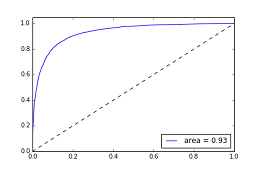
\includegraphics{images/pvdmconcat.png}
	\caption{Courbe ROC pour le modèle PC-DM avec concaténation.}
	\label{pcdmconcat}
	\end{center}
	\end{figure}
	\end{frame}
	
	\begin{frame}
	\begin{figure}[h]
\begin{center}
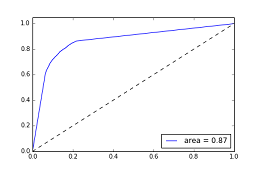
\includegraphics{images/pvdmmean.png}
\caption{Courbe ROC pour le modèle PC-DM avec moyenne.}
\label{pcdmmean}
\end{center}
\end{figure}
	\end{frame}

\subsection{Derniers essais}

\begin{frame}
Finalement, nous avons concaténé les vecteurs de paragraphes et les vecteurs obtenus à partir des n-grammes. Nous obtenons une précision de $0.90116$.
\end{frame}

\begin{frame}{Conclusion}
\begin{center}
{\Huge Merci !}
\end{center}
\end{frame}

\end{document}